\documentclass[
      aspectratio=169,
        12pt,
    ]{beamer}

% font
\usefonttheme[onlymath]{serif}
\usepackage[T1]{fontenc}
\usepackage{textcomp}
\usepackage[scale = 1.0]{tgheros} %Sans serif
\usepackage[scaled]{beramono}
\usepackage{luatexja-otf}
\usepackage[match, deluxe, expert, noto-otf]{luatexja-preset}
\renewcommand{\kanjifamilydefault}{\gtdefault}

% math packages
\usepackage{amsmath,amssymb}
\usepackage{siunitx}

% comment out package
\usepackage{comment}

% tables
\usepackage{longtable, booktabs, array}
\usepackage{threeparttable, threeparttablex, multirow}
\newcolumntype{d}{S[input-symbols = ()]}

% figures
\usepackage{graphics, graphicx}
\makeatletter
\def\maxwidth{\ifdim\Gin@nat@width>\linewidth\linewidth\else\Gin@nat@width\fi}
\def\maxheight{\ifdim\Gin@nat@height>\textheight\textheight\else\Gin@nat@height\fi}
\makeatother
% Scale images if necessary, so that they will not overflow the page
% margins by default, and it is still possible to overwrite the defaults
% using explicit options in \includegraphics[width, height, ...]{}
\setkeys{Gin}{width=\maxwidth,height=\maxheight,keepaspectratio}

% navigation symbol
\setbeamertemplate{navigation symbols}{}

% page numbers
\setbeamertemplate{footline}[frame number]

% itemize
\setbeamercolor{item}{fg=black}
\setbeamertemplate{itemize item}[circle]
\setbeamertemplate{itemize subitem}[circle]
\setbeamertemplate{itemize subsubitem}[circle]

\providecommand{\tightlist}{%
  \setlength{\itemsep}{0pt}\setlength{\parskip}{0pt}}

% title design
\setbeamerfont{title}{size=\Large,series=\bfseries}
\setbeamerfont{subtitle}{series=\bfseries}
\setbeamerfont{frametitle}{size=\Large,series=\bfseries}

% header includes

% Title information
  \title{骨髄バンクナッジ介入実験}
  \subtitle{解析結果途中報告}
  \author{%
        加藤 大貴
    \and
      }

\begin{document}

\frame{\titlepage}

\begin{frame}
\end{frame}

\begin{frame}{フィールド実験の介入}
\protect\hypertarget{ux30d5ux30a3ux30fcux30ebux30c9ux5b9fux9a13ux306eux4ecbux5165}{}
\begin{itemize}
\tightlist
\item
  対象:骨髄バンクドナー確定後に「適合通知」を受け取るドナー候補者(\(N = 11,154\))
\item
  ドナー候補者確定後、骨髄バンクは対象者に幹細胞提供を依頼する「適合通知」および
  それを郵送した旨を伝えるSNSメーセージを送付
\item
  行動科学の知見に基づいたメッセージを適合通知に加える介入を実施E
\end{itemize}
\end{frame}

\begin{frame}{通常の適合通知の内容}
\protect\hypertarget{ux901aux5e38ux306eux9069ux5408ux901aux77e5ux306eux5185ux5bb9}{}
\begin{quote}
この度、あなたと骨髄バンクの登録患者さんのHLA型(白血球の型)が一致し、
ドナー候補者のおひとりに選ばれました。
今後、ご提供に向け詳しい検査や面談を希望されるかをお伺いしたく連絡させていただきました。
同封の資料をよくお読みいただき、コーディネートが可能かどうか検討の上、
この案内が届いてから7日以内に返信用紙ほかをご返送ください。
返送後、コーディネートを進めさせていただく場合は、
担当者よりご相談のお電話を差し上げますのでよろしくお願い申し上げます。
\end{quote}
\end{frame}

\begin{frame}{介入内容}
\protect\hypertarget{ux4ecbux5165ux5185ux5bb9}{}
\begin{enumerate}
[a.]
\tightlist
\item
  確率メッセージ:「1人の登録患者さんとHLA型が一致するドナー登録者は数百〜数万人に1人です。
  ドナー候補者が複数みつかる場合もありますが、多くはないこともご理解頂ければ幸いです。」
\item
  移植患者情報:「骨髄バンクを介して移植ができる患者さんは現在約6割にとどまっています。
  骨髄等を提供するドナーが早く見つかれば、その比率を高めることができます。」
\end{enumerate}
\end{frame}

\begin{frame}{実験群}
\protect\hypertarget{ux5b9fux9a13ux7fa4}{}
\begin{itemize}
\tightlist
\item
  A群(コントロール):通常の適合通知
\item
  B群(トリートメント1):通常の適合通知+確率メッセージ
\item
  C群(トリートメント2):通常の適合通知+移植患者情報
\item
  D群(トリートメント3):通常の適合通知+確率メッセージ+移植患者情報
\end{itemize}
\end{frame}

\begin{frame}{介入スケジュール}
\protect\hypertarget{ux4ecbux5165ux30b9ux30b1ux30b8ux30e5ux30fcux30eb}{}
週・月の固定効果を取り除くために、実験群は月・週でバランスするように週単位で割り当てた

\begin{table}
\centering
\begin{tabular}[t]{ccccccc}
\toprule
\multicolumn{1}{c}{ } & \multicolumn{6}{c}{月/年} \\
\cmidrule(l{3pt}r{3pt}){2-7}
週 & 9/21 & 10/21 & 11/21 & 12/21 & 1/22 & 2/22\\
\midrule
1 & B & C & C & D & B & A\\
2 & D & B & A & A & C & B\\
3 & A & D & B & C & D & C\\
4 & C & A & D & B & A & D\\
\bottomrule
\end{tabular}
\end{table}
\end{frame}

\begin{frame}{フィールド実験概要}
\protect\hypertarget{ux30d5ux30a3ux30fcux30ebux30c9ux5b9fux9a13ux6982ux8981}{}
\begin{table}
\centering
\begin{tabular}[t]{lccccc}
\toprule
\multicolumn{1}{c}{ } & \multicolumn{4}{c}{実験群} & \multicolumn{1}{c}{ } \\
\cmidrule(l{3pt}r{3pt}){2-5}
  & A & B & C & D & p-value\\
\midrule
\addlinespace[0.3em]
\multicolumn{6}{l}{\textbf{A. 介入}}\\
\hspace{1em}通常の適合通知 & X & X & X & X & \\
\hspace{1em}確率メッセージ &  & X &  & X & \\
\hspace{1em}移植患者情報 &  &  & X & X & \\
\addlinespace[0.3em]
\multicolumn{6}{l}{\textbf{B. サンプルサイズ}}\\
\hspace{1em}サンプルサイズ & 2558 & 3075 & 2754 & 2766 & \\
\addlinespace[0.3em]
\multicolumn{6}{l}{\textbf{C. 共変量}}\\
\hspace{1em}年齢 & \num{38.37} & \num{38.13} & \num{37.43} & \num{37.99} & \num{0.06}\\
\hspace{1em}過去のコーディネーション回数 & \num{1.61} & \num{1.59} & \num{1.63} & \num{1.56} & \num{0.36}\\
\hspace{1em}1 = 男性 & \num{0.62} & \num{0.63} & \num{0.63} & \num{0.61} & \num{0.40}\\
\bottomrule
\end{tabular}
\end{table}
\end{frame}

\begin{frame}{アウトカム変数}
\protect\hypertarget{ux30a2ux30a6ux30c8ux30abux30e0ux5909ux6570}{}
アウトカム変数は提供に至るまでのプロセスであり、具体的に以下の6つの工程がある。

\begin{itemize}
\tightlist
\item
  Reply: 適合通知に返信したならば1を取る二値変数
\item
  Intention: 提供を希望するという意向を示して返信したならば1を取る二値変数
\item
  CT: 確認検査を実施したならば1を取る二値変数
\item
  Candidate: 第一候補者に選定されたならば1を取る二値変数
\item
  Consent: 最終同意をしたならば1を取る二値変数
\item
  Donation: 採取をしたならば1を取る二値変数
\end{itemize}
\end{frame}

\begin{frame}{返信~確認検査の二群比較の検定}
\protect\hypertarget{ux8fd4ux4fe1ux78baux8a8dux691cux67fbux306eux4e8cux7fa4ux6bd4ux8f03ux306eux691cux5b9a}{}
\begin{center}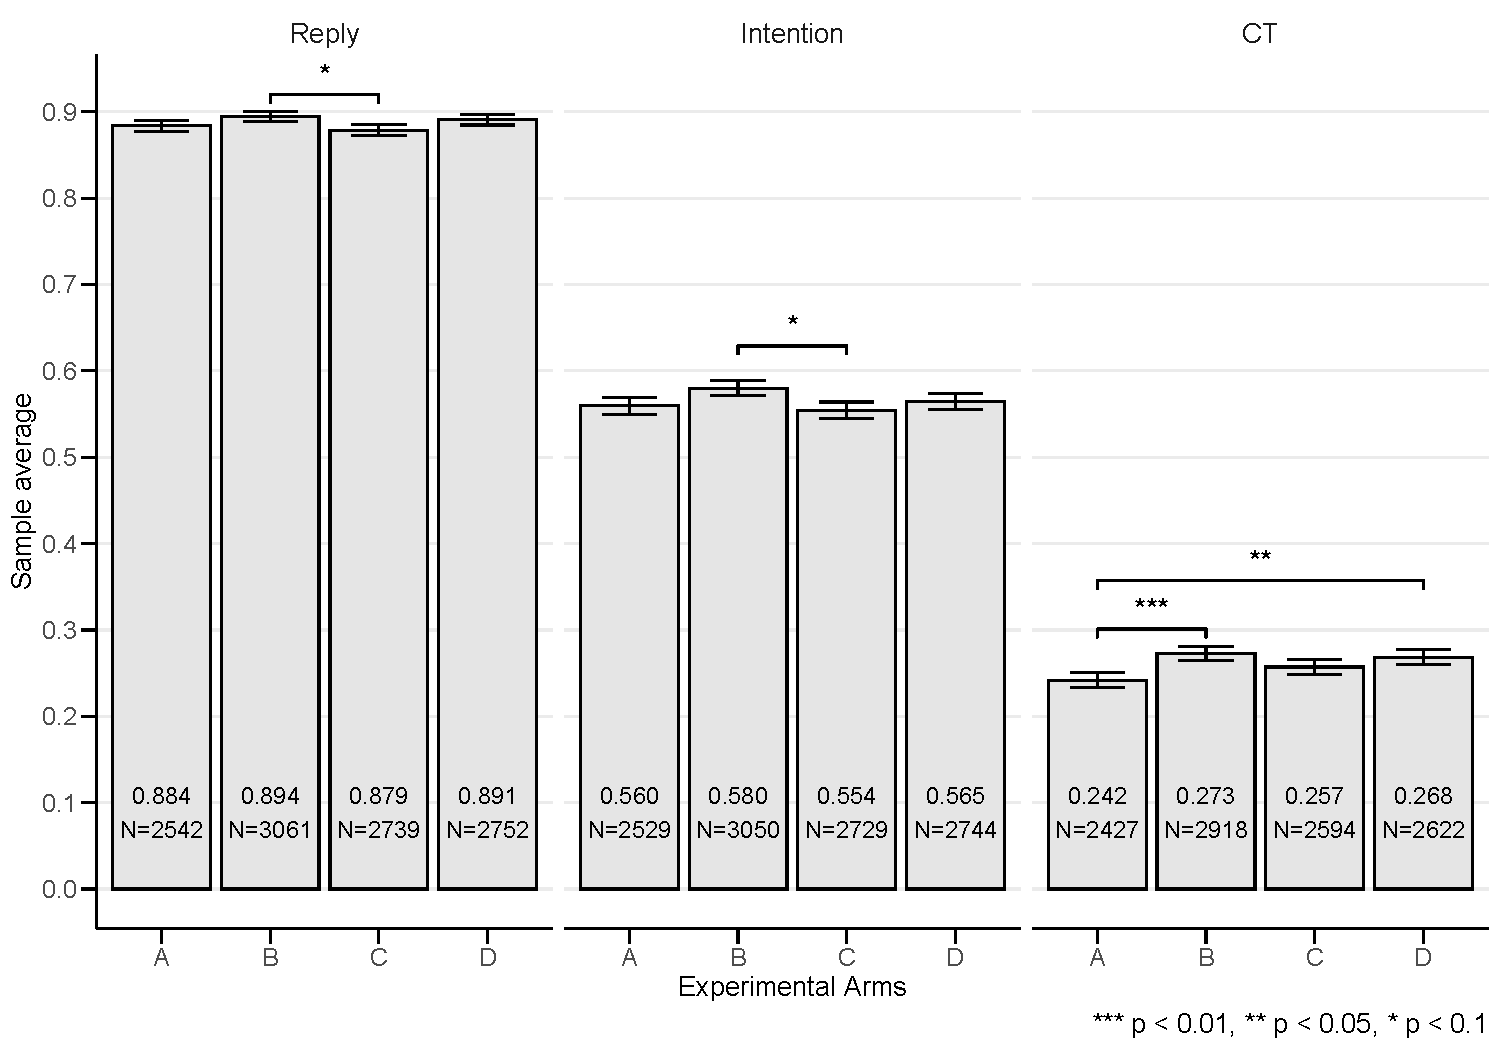
\includegraphics[width=0.75\linewidth]{report_files/figure-beamer/ttest-1-3step-1} \end{center}
\end{frame}

\begin{frame}{候補者選定~採血までの二群比較の検定}
\protect\hypertarget{ux5019ux88dcux8005ux9078ux5b9aux63a1ux8840ux307eux3067ux306eux4e8cux7fa4ux6bd4ux8f03ux306eux691cux5b9a}{}
\begin{center}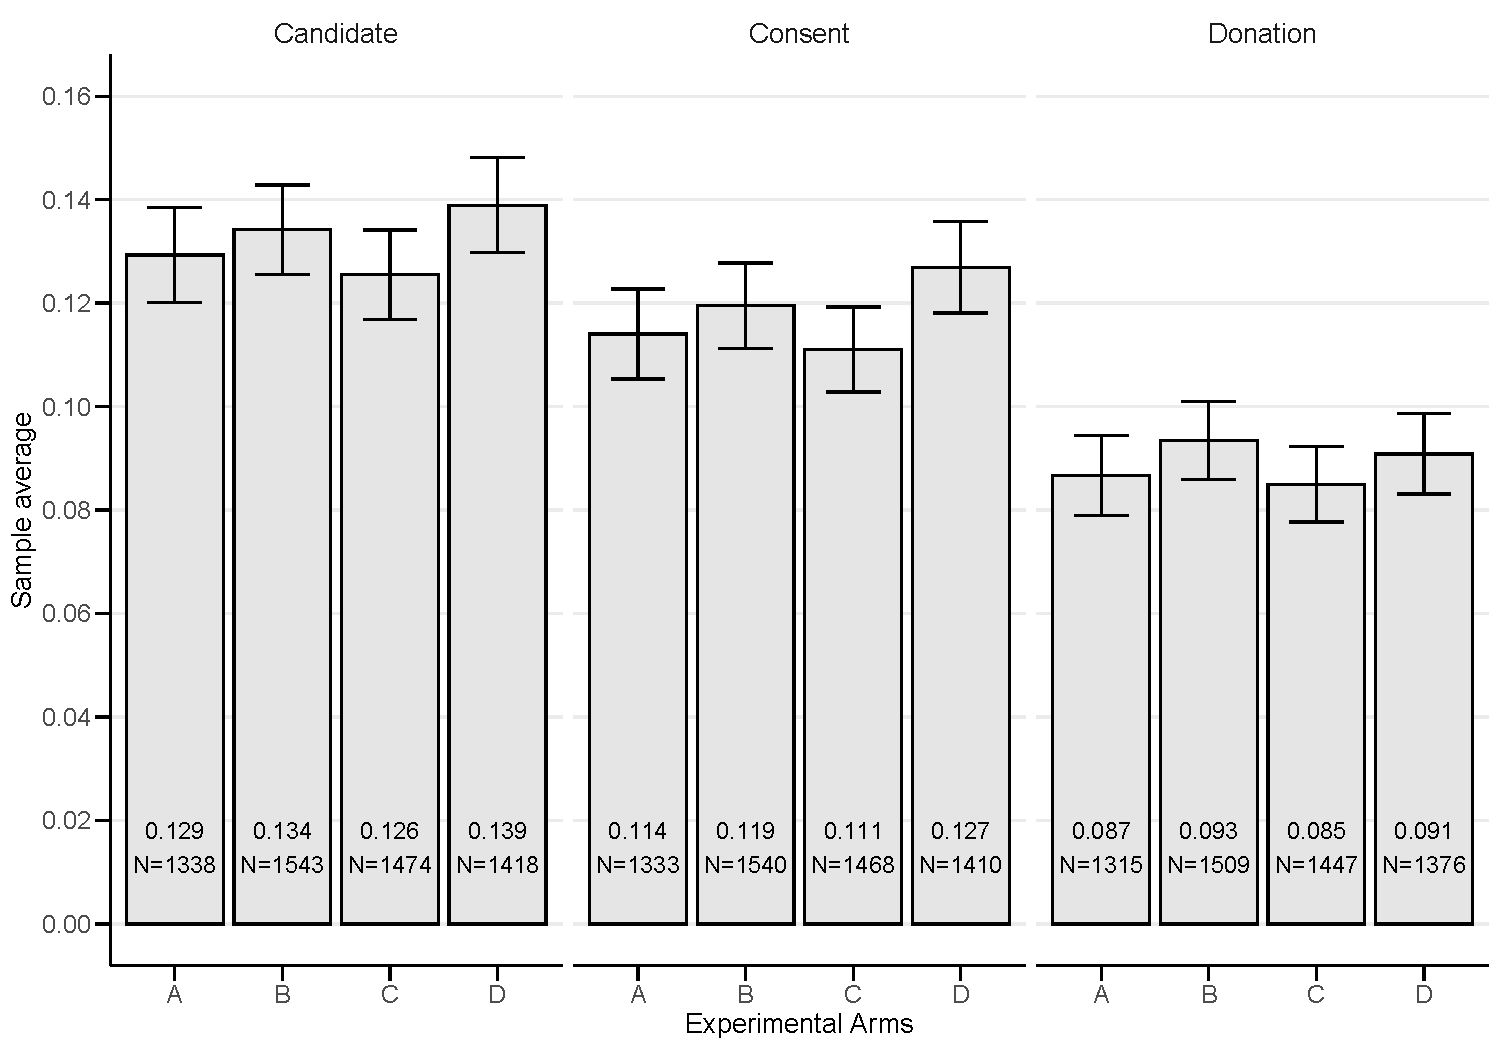
\includegraphics[width=0.75\linewidth]{report_files/figure-beamer/ttest-4-6step-1} \end{center}
\end{frame}

\begin{frame}{線形確率モデル}
\protect\hypertarget{ux7ddaux5f62ux78baux7387ux30e2ux30c7ux30eb}{}
\(m\)月の第\(w\)週に適合通知を受け取った個人\(i\)について、

\[
  Y_{imw} =
  \beta_1 \cdot \text{B}_{mw} + \beta_2 \cdot \text{C}_{mw}
  + \beta_3 \cdot \text{D}_{mw}
  + X'_i \gamma + \lambda_m + \theta_w + u_{imw}
\]

\begin{itemize}
\tightlist
\item
  \(X_i\)は性別・年齢・居住する都道府県・コーディネーション回数
\item
  \(\lambda_m\)と\(\theta_w\)は週・月の固定効果
\end{itemize}
\end{frame}

\begin{frame}{モデル推定結果}
\protect\hypertarget{ux30e2ux30c7ux30ebux63a8ux5b9aux7d50ux679c}{}
\begin{table}
\centering
\fontsize{9}{11}\selectfont
\begin{tabular}[t]{l>{\centering\arraybackslash}p{5em}>{\centering\arraybackslash}p{5em}>{\centering\arraybackslash}p{5em}>{\centering\arraybackslash}p{5em}>{\centering\arraybackslash}p{5em}>{\centering\arraybackslash}p{5em}}
\toprule
  & Reply & Intention & CT & Candidate & Consent & Donation\\
\midrule
B & \num{0.013}** & \num{0.019} & \num{0.034}*** & \num{0.002} & \num{0.002} & \num{0.003}\\
 & (\num{0.006}) & (\num{0.013}) & (\num{0.009}) & (\num{0.009}) & (\num{0.007}) & (\num{0.007})\\
C & \num{0.002} & \num{-0.005} & \num{0.015} & \num{-0.010} & \num{-0.009} & \num{-0.007}\\
 & (\num{0.005}) & (\num{0.011}) & (\num{0.010}) & (\num{0.009}) & (\num{0.007}) & (\num{0.008})\\
D & \num{0.006} & \num{0.006} & \num{0.032}*** & \num{0.008} & \num{0.011} & \num{0.002}\\
 & (\num{0.005}) & (\num{0.010}) & (\num{0.010}) & (\num{0.008}) & (\num{0.007}) & (\num{0.008})\\
\midrule
Num.Obs. & \num{11093} & \num{11051} & \num{10560} & \num{5772} & \num{5750} & \num{5646}\\
\addlinespace[0.3em]
\multicolumn{7}{l}{\textit{F-tests, p-value}}\\
\hspace{1em}B = C & \num{0.015} & \num{0.007} & \num{0.084} & \num{0.293} & \num{0.230} & \num{0.152}\\
\hspace{1em}B = D & \num{0.233} & \num{0.114} & \num{0.856} & \num{0.495} & \num{0.325} & \num{0.917}\\
\hspace{1em}C = D & \num{0.277} & \num{0.164} & \num{0.148} & \num{0.068} & \num{0.018} & \num{0.220}\\
\bottomrule
\multicolumn{7}{l}{\rule{0pt}{1em}* p $<$ 0.1, ** p $<$ 0.05, *** p $<$ 0.01}\\
\end{tabular}
\end{table}
\end{frame}

\begin{frame}{返信スピードに対する効果}
\protect\hypertarget{ux8fd4ux4fe1ux30b9ux30d4ux30fcux30c9ux306bux5bfeux3059ux308bux52b9ux679c}{}
ログランク検定:chi-square = 0.883; p-value = 0.829

\begin{center}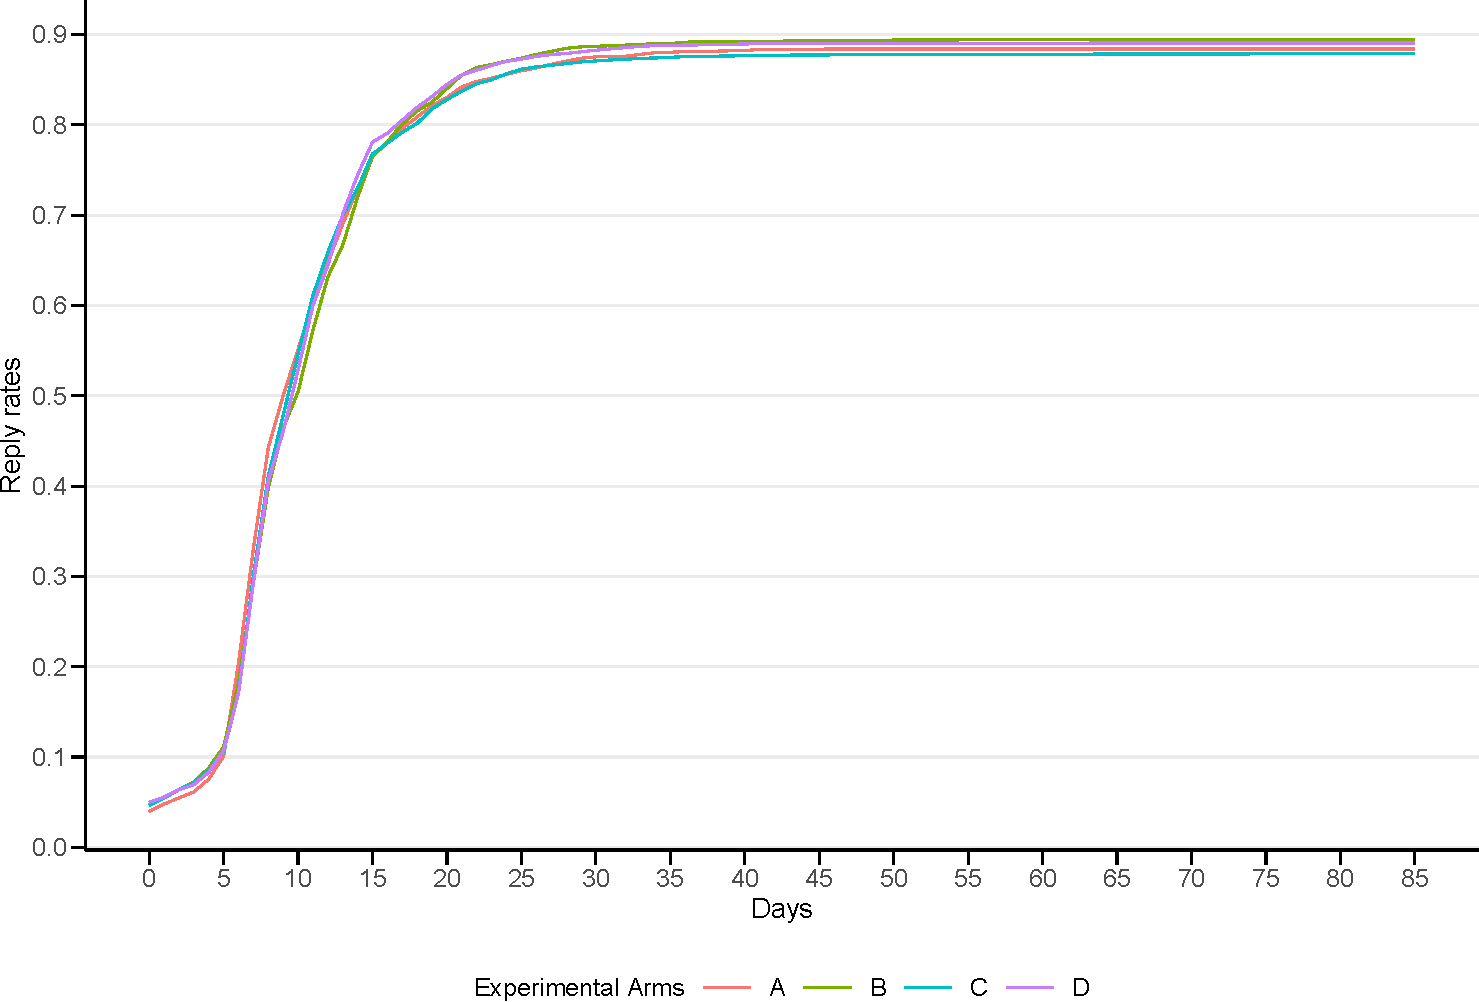
\includegraphics[width=0.75\linewidth]{report_files/figure-beamer/plot-reply-speed-1} \end{center}
\end{frame}

\begin{frame}{特定日数までの返信に対する効果}
\protect\hypertarget{ux7279ux5b9aux65e5ux6570ux307eux3067ux306eux8fd4ux4fe1ux306bux5bfeux3059ux308bux52b9ux679c}{}
\begin{table}
\centering
\fontsize{9}{11}\selectfont
\begin{tabular}[t]{l>{\centering\arraybackslash}p{5em}>{\centering\arraybackslash}p{5em}>{\centering\arraybackslash}p{5em}>{\centering\arraybackslash}p{5em}>{\centering\arraybackslash}p{5em}}
\toprule
\multicolumn{1}{c}{ } & \multicolumn{1}{c}{≦ 10days} & \multicolumn{1}{c}{≦ 20days} & \multicolumn{1}{c}{≦ 30days} & \multicolumn{1}{c}{≦ 40days} & \multicolumn{1}{c}{≦ 85days} \\
\cmidrule(l{3pt}r{3pt}){2-2} \cmidrule(l{3pt}r{3pt}){3-3} \cmidrule(l{3pt}r{3pt}){4-4} \cmidrule(l{3pt}r{3pt}){5-5} \cmidrule(l{3pt}r{3pt}){6-6}
  & (1) & (2) & (3) & (4) & (5)\\
\midrule
B & \num{-0.044}*** & \num{0.013} & \num{0.015}** & \num{0.012}* & \num{0.013}**\\
 & (\num{0.014}) & (\num{0.009}) & (\num{0.007}) & (\num{0.006}) & (\num{0.006})\\
C & \num{0.002} & \num{0.007} & \num{0.004} & \num{0.001} & \num{0.002}\\
 & (\num{0.015}) & (\num{0.007}) & (\num{0.006}) & (\num{0.005}) & (\num{0.005})\\
D & \num{-0.028}* & \num{0.018}** & \num{0.007} & \num{0.007} & \num{0.006}\\
 & (\num{0.014}) & (\num{0.007}) & (\num{0.005}) & (\num{0.005}) & (\num{0.005})\\
\midrule
Num.Obs. & \num{11093} & \num{11093} & \num{11093} & \num{11093} & \num{11093}\\
\addlinespace[0.3em]
\multicolumn{6}{l}{\textit{F-tests, p-value}}\\
\hspace{1em}B = C & \num{0.004} & \num{0.282} & \num{0.028} & \num{0.021} & \num{0.015}\\
\hspace{1em}B = D & \num{0.259} & \num{0.474} & \num{0.135} & \num{0.351} & \num{0.233}\\
\hspace{1em}C = D & \num{0.064} & \num{0.022} & \num{0.463} & \num{0.165} & \num{0.277}\\
\bottomrule
\multicolumn{6}{l}{\rule{0pt}{1em}* p $<$ 0.1, ** p $<$ 0.05, *** p $<$ 0.01}\\
\end{tabular}
\end{table}
\end{frame}

\end{document}
